\section{Rappresentazione grafica della simulazione}
La visualizzazione della simulazione è stata realizzata utilizzando un Web
Server, appositamente realizzato per lo scopo, e tecnologie web per la
realizzazione di contenuti web quali HTML5, JavaScript e WebSocket.
Gli utenti del sistema possono assistere alla simulazione semplicemente
visualizzando un'apposita pagina web nel loro browser.

Nel sistema di visualizzazione si possono identificare due componenti
principali: un web server e la pagina web caricata dal singolo visualizzatore.
I compiti principali del web server sono quelli di interfacciarsi con il resto
del sistema, fornire agli utenti un punto da cui poter reperire le pagine per la
visualizzazione della simulazione e inoltrare gli aggiornamenti di stato dal
sistema ai vari client.
Infine, la pagina web caricata nel browser (client) ha il compito di ricevere
gli stati della simulazione e di rappresentarli graficamente all'utente.

\subsection{Requisiti}\label{subsec:requisiti}
L'interfaccia grafica è stata progettata e realizzata in modo tale da
soddisfare una serie di requisiti che derivano dalla natura distribuita del
sistema. 

\begin{description}
	\item[Scalabilità:] la rappresentazione grafica della simulazione deve 
	adattarsi alla dimensione del sistema. Deve essere garantita la possibilità 
	di visualizzare nel dettaglio lo stato di ogni singolo quartiere simulato dal
	sistema.

	\item[Coerenza:] la rappresentazione attuale della simulazione deve essere
	coerente con lo stato attuale del sistema. Nel dettaglio, la rappresentazione
	della posizione degli abitanti dei quartieri deve essere fedele con la
	posizione effettiva nella simulazione. Questa condizione viene rilassata per
	permettere l'utilizzo di tecniche che rendono la visualizzazione più fluida.
	
	\item[Utilità:] oltre a visualizzare la simulazione, l'interfaccia grafica deve
	essere utilizzabile per la verifica e il controllo delle mappe in fase di
	sviluppo. Data la descrizione degli elementi presenti in un quartiere, la
	libreria di visualizzazione deve essere in grado di fornire tutte le misure
	necessarie al sistema per eseguire la simulazione.
	
	\item[Flessibilità:] una caratteristica del sistema è la sua flessibilità e
	configurabilità. La visualizzazione deve adattarsi a questa caratteristica e in
	particolar modo deve permettere la descrizione della mappa in modo flessibile e
	facile da modificare.
	
\end{description}

\subsection{Web server}
Lo scopo principale del web server è quello di fare da ponte tra il sistema che
esegue la simulazione e il client che ne visualizza lo stato.

Nel dettaglio, i compiti svolti da questo componente sono:
\begin{itemize}
	\item ricevere le descrizioni di tutte le mappe rappresentanti i quartieri,
	fornite dai singoli nodi che eseguono la simulazione;
	\item fornire una pagina principale per la selezione del quartiere da
	osservare;
	\item mettere a disposizione dei client le descrizioni di tutte le mappe
	registrate;
	\item inoltrare gli aggiornamenti di stato relativi ad un quartiere verso i
	client che ne osservano la simulazione;
	\item ricevere richieste di terminazione dai client e inoltrarli al resto del
	sistema;
	\item notificare i client della terminazione della simulazione.
\end{itemize}

\subsubsection{Interfacce}
Il web server prevede due interfacce principali: una con il resto del sistema e
una con i client che vengono avviati dagli utenti.

\paragraph*{Interfaccia con il sistema di simulazione}
Questa interfaccia elenca le funzionalità messe a disposizione al resto del
sistema da parte del web server.

Le funzioni disponibili sono descritte di seguito.
\begin{description}
	\item[registra\_mappa\_quartiere:] permette ad un nodo che gestisce un
	quartiere di registrare la propria mappa presso il web server. In seguito alla
	chiamata di questo metodo, il web server predisporrà le risorse necessarie per
	permettere ai client di visualizzare la simulazione del quartiere appena
	registrato.
	\item[invia\_aggiornamento:] permette ad un nodo che gestisce un quartiere di
	inviare ai client che osservano la zona in questione i relativi aggiornamenti
	di stato.
	\item[close\_webserver:] notifica a tutti i client che la simulazione è stata
	terminata. Una volta notificati tutti i client, il web server viene terminato.
\end{description}

\paragraph*{Interfaccia con i client}
Per permettere ai client di ottenere informazioni riguardanti la simulazione, il
web server mette a disposizione una serie di risorse web accessibili tramite
protocollo HTTP. 

La risorsa principale è raggiungibile visitando l'indirizzo del server con un
web browser.
La pagina principale elenca il numero massimo di quartieri ammessi nella
simulazione e, tra questi, quelli attualmente attivi. Lo stato globale della
simulazione è visualizzato in scala ridotta e solamente i veicoli sono
rappresentati nelle strade.

Le pagine che permettono di visualizzare lo stato di un singolo quartiere sono
raggiungibili visitando la risorsa identificata dall'URL avente come hostname
l'indirizzo del server e come percorso la parola ``quartiere'' immediatamente
seguita dall'id del quartiere di interesse. Ad esempio, se il server è attivo su
\texttt{localhost} e siamo interessati al quartiere con id 2 dovremo usare l'URL
\url{http://localhost/quartiere2}.

Ogni quartiere attivo fornisce l'accesso a due ulteriori risorse: la mappa e uno
canale tramite il quale vengono forniti gli aggiornamenti.
La mappa è reperibile aggiungendo \texttt{/map.json} al percorso utilizzato per
accedere alla pagina del quartiere (\url{http://localhost/quartiere2/map.json}).
Gli aggiornamenti di stato sono ottenibili aprendo un WebScoket verso l'URL del
relativo al quartiere di interesse, al quale viene aggiunto
\texttt{/updatesStream} (\url{http://localhost/quartiere2/updatesStream}).

\subsubsection{Ciclo di vita}
Il ciclo di vita del web server è caratterizzato da diverse fasi operative,
descritte di seguito.

\begin{description}
	\item[Avvio:] il web server viene avviato assieme al resto delle componenti del
	sistema.
	\item[Inizializzazione:] questa procedura chiede al name server il numero
	massimo di quartieri facenti parte della simulazione e alloca le risorse
	necessarie al webserver per eseguire. Una volta inizializzate le risorse il web
	server viene avviato e risulta raggiungibile dai client.
	\item[Registrazione:] il secondo passo è quello di registrare il web server
	presso il name server. In questo modo le varie partizioni potranno ottenere un
	riferimento al web server.
	\item[Fase operativa:] durante questa fase il web server è raggiungibile sia
	dai client che dalle partizioni che gestiscono i quartieri. Le partizioni
	registreranno la propria mappa utilizzando il metodo
	\texttt{registra\_mappa\_quartiere}. Questa procedura comporterà il salvataggio
	presso il web server della mappa del quartiere e l'inizializzazione della
	relativa pagina web e gestore dei WebSocket. A questo punto la partizione può
	inviare al web server gli aggiornamenti di stato, i quali saranno inoltrati ai
	client registrati per essi, attraverso l'opportuno WebSocket.
	I client possono accedere alle pagine dei quartieri attivi già registrati e
	attivare un WebSocket per ricevere gli aggiornamenti di stato.
	Durante questa fase un client può inoltrare, attraverso lo stesso WebSocket, la
	richiesta di terminazione della simulazione.
	\item[Terminazione:] la simulazione, e quindi anche la sua visualizzazione,
	viene terminata in seguito alla richiesta da parte di un client. Il web server
	ha il compito di attendere la richiesta di terminazione da parte di un client e
	inoltrarla al name server. Prima di notificare il name server, il web server
	avverte tutti i client dell'imminente terminazione della simulazione.
	A terminazione avvenuta, il name server notifica il web server della fine della
	simulazione usando il metodo \texttt{close\_webserver}. Questa procedura causa
	la notifica a tutti i client dell'avvenuta fine della simulazione.
	Successivamente il web server viene spento, liberando tutte le risorse utilizzate ed eliminando
	eventuali file temporanei. L'ultima azione consiste nel notificare il name
	server dell'avvenuto spegnimento. La Figura \ref{fig:stopwebserver} descrive
	questa procedura.
\end{description}

\begin{figure}[H] % Example image
\center{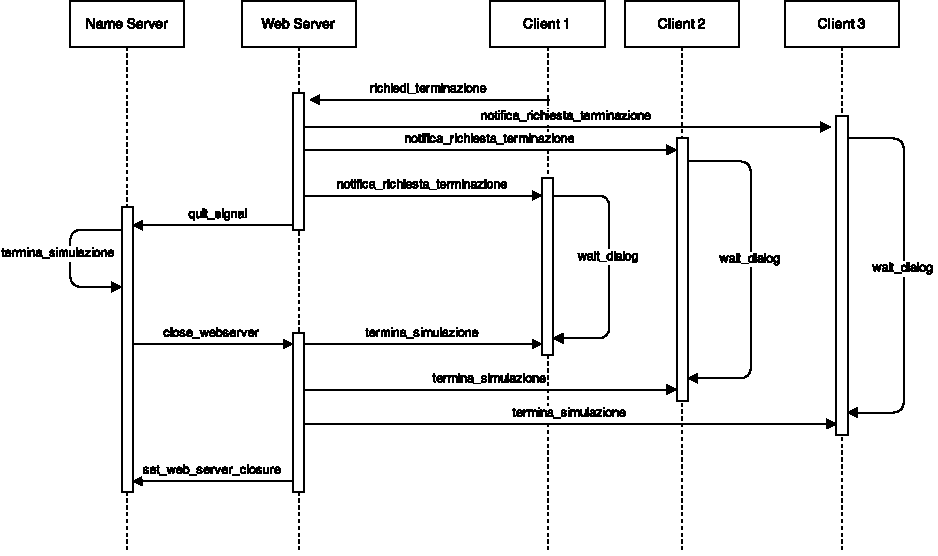
\includegraphics[width=\linewidth]{ChiusuraWebServer}}
\caption{Diagramma di sequenza che descrive la procedura di terminazione della
visualizzazione della simulazione}
\label{fig:stopwebserver}
\end{figure}

\subsection{Client}
Il client ha la possibilità di eseguire tre funzionalità differenti,
implementate ognuna in una pagina web specifica:
\begin{itemize}
	\item visualizzazione della lista dei quartieri attivi e situazione globale
	della simulazione
	\item visualizzazione della simulazione di un quartiere
	\item supporto allo sviluppo e preprocessamento dei file di descrizione delle
	mappe
\end{itemize}

\subsubsection{Definizione della mappa}
Il file di definizione della mappa contiene tutte le informazioni necessarie per
eseguire la simulazione di un singolo quartiere. 

L'unità di misura utilizzata nella definizione dei vari elementi è il metro, che
in fase di visualizzazione corrisponderà inizialmente con un pixel sullo
schermo.

All'interno del file di definizione si trovano le descrizioni di:
\begin{itemize}
	\item strade urbane;
	\item strade di ingresso;
	\item incroci con 3 e 4 strade incidenti (descritti separatamente);
	\item luoghi.
\end{itemize}

In aggiunta a quanto elencato sopra, vi si trovano anche informazioni
riguardanti il quartiere e le entità che si muovono in esso (pedoni, bici, auto
e bus).

Di seguito descriveremo le caratteristiche di ogni singola entità.

\paragraph*{Strade urbane}
Le strade urbane sono l'entità principale della definizione della mappa. Sono
caratterizzate da un identificativo numerico e dalla loro posizione all'interno
del quartiere. 

Il sistema di coordinate utilizzato per definire i punti all'interno della mappa
ha l'origine degli assi nell'angolo più in alto a sinistra.

 La posizione della strada è definita da due attributi: \texttt{from} e
 \texttt{to}, ovvero il punto in cui inizia e in cui finisce.
Per questi due valori è stata concordata la seguente convenzione: l'estremo
\texttt{from} è quello avente coordinata x con valore minore. In caso i valori
x dei due estremi siano uguali, l'estremo \texttt{from} è quello avente la y
minore.
Un esempio di questa convenzione è rappresentato in Figura
\ref{fig:polaritastrade}.

\begin{figure}[H] % Example image
\center{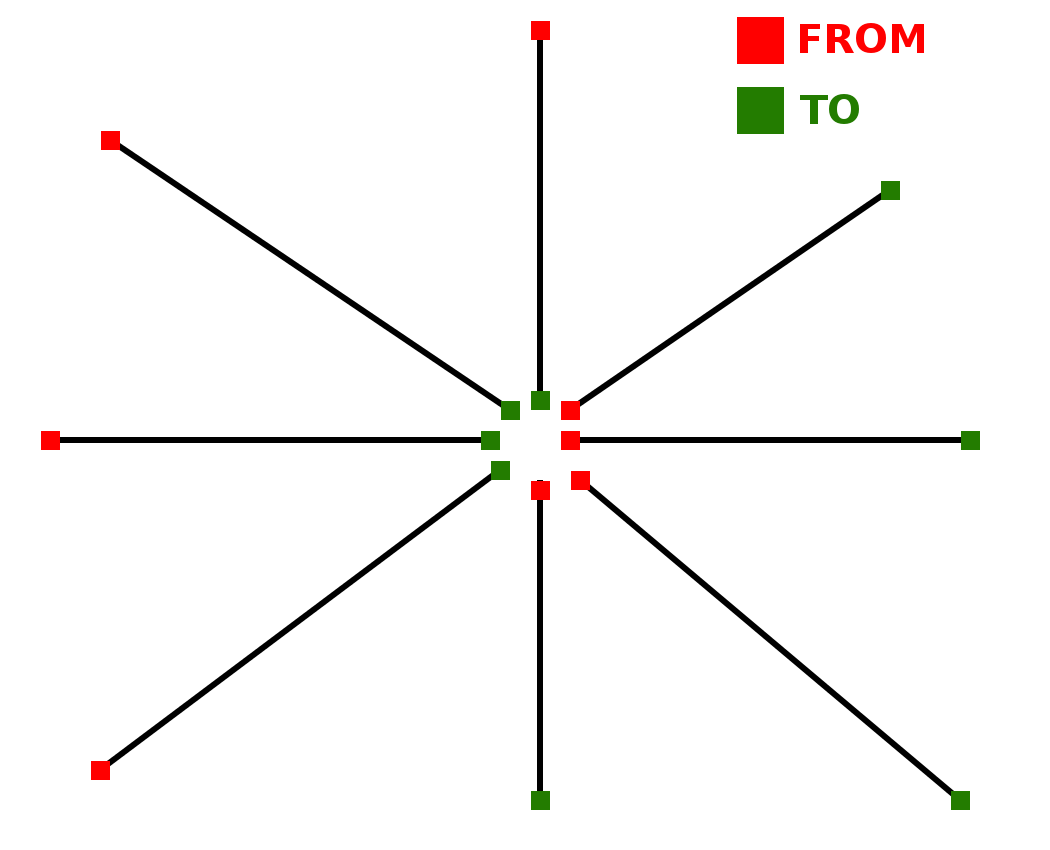
\includegraphics[width=0.8\linewidth]{polarita_strade}}
\caption{Convenzione per la definizione delle coordinate delle strada.}
\label{fig:polaritastrade}
\end{figure}

All'estremo \texttt{from} è associato il valore booleano \texttt{true} mentre
all'estremo \texttt{to} il valore \texttt{false}.
Questa convenzione ci permette di definire in modo univoco come una entità
percorre una strada: le entità viaggiano, da un estremo all'altro di una strada,
utilizzando le corsie o i marciapiedi a destra della linea di mezzaria. Il lato
della strada percorso da una entità è identificato dal valore booleano
dell'estremo verso cui ci si sta dirigendo. Ad esempio, se una macchina si sta
muovendo dall'estremo \texttt{to} all'estremo \texttt{from} allora sta
percorrendo il lato \texttt{true} della strada.

La forma effettiva della strada verrà definita in fase di rendering. Per questo
motivo, la lunghezza effettiva della strada deve essere calcolata processando il
file di descrizione con l'apposita applicazione client.

Ogni strada urbana può definire un numero arbitrario di corsie per senso di
marcia.
Per la realizzazione di questo sistema è stato scelto di fissare questo valore a 2.

\paragraph*{Strade di ingresso}
Le strade di ingresso sono le rappresentazioni dei viali o strade di accesso a
case o edifici. Come le strade urbane, possiedono un identificativo ma sono
prive di estremi \texttt{from} e \texttt{to}.
Per convenzione sono sempre strade prive di curve e sono posizionate in
riferimento ad una strada principale. Per questo motivo, la posizione di queste
strade è definita utilizzando l'id della strada urbana a cui si riferiscono, il
lato della strada dove si immettono e la distanza in metri dall'estremo
\texttt{from}.

Anche questo tipo di strada ammette un parametro che specifica il numero di
corsie per il senso di marcia. Analogamente alle strade urbane, questo è fisso
per la simulazione ed è settato a 1.

\paragraph*{Incroci}
Per motivi di semplicità di realizzazione del sistema di simulazione, si è
distinto tra incroci aventi 4 strade incidenti e incroci aventi 3 strade
incidenti. 

Ogni definizione di incrocio contiene un identificativo e una lista delle strade
incidenti all'incrocio. Per convenzione la prima strada è quella che entra
nell'incrocio da nord, le successive sono quelle che seguono in senso orario.

Gli incroci a tre ingressi presentano un campo addizionale che indica quale
delle strade incidenti non è presente.

Per ogni strada incidente ad un incrocio viene indicato l'identificativo del
quartiere, l'identificativo della strada, il tipo e l'estremo che si affaccia
nell'incrocio.

\paragraph*{Luoghi}
L'ultimo elemento rappresentato nella mappa sono i luoghi. Un luogo può
rappresentare una casa privata, un luogo di lavoro, un qualsiasi edificio o una
fermata per autobus. 

Ogni luogo presenta un identificativo, un nome ed una tipologia. Il
posizionamento viene eseguito utilizzando l'identificativo della relativa strada
di ingresso e delle dimensioni, anch'esse specificate nella definizione del
luogo. Ulteriori dettagli specificano la capienza del luogo in termine di
persone, auto e bici.

\subsubsection{Rappresentazione della mappa}
La rappresentazione grafica della mappa, a partire dalla descrizione di un
quartiere, procede prima caricando tutti gli elementi da visualizzare e poi
disegnandoli effettivamente sullo schermo.

La rappresentazione grafica è realizzata mediante la libreria
Paper.js~\cite{paperjs}, la quale permette di semplificare notevolmente le
operazioni di disegno su di un oggetto Canvas.

Tutte le fasi di caricamento e disegno della mappa vengono eseguite attraverso
uno specifico oggetto JavaScript. Quest'ultimo funge anche da registro per
le strade, incroci e altre entità statiche della mappa.

La prima fase consiste nel creare le istanze degli oggetti strada, incrocio e
lugo, caricarle nei registri e poi collegarle tra loro. La fase di collegamento
è cruciale: le strade di ingresso devono conoscere la posizione della strada
principale a cui sono collegate e gli incroci devono conoscere le strade a loro
incidenti per risolvere la posizione dell'incrocio stesso.

La fase successiva prevede il disegno vero e proprio delle entità sullo schermo.
Le strade incidenti agli incroci, una volta collegate, vengono alterate in modo
da modificarne la forma. Questa operazione permette di inserire curvature che
rendono la strada meno seghettata e più realistica.
Questa fase comprende anche la creazione delle traiettorie utilizzate dalla
simulazione, come descritto nella Sezione \ref{subsec:protocolloavanzamento}.
Tutte le traiettorie vengono indicizzate in modo da essere facilmente reperite
in un secondo momento.

La rappresentazione grafica della mappa non è utilizzata solamente durante la
visualizzazione della simulazione: lo strumento di aiuto allo sviluppo delle
mappe permette di visualizzare la mappa che si sta creando e di calcolare le
lunghezze effettive di strada e traiettorie.
Una volta elaborato con questo strumento, è possibile utilizzare un file di
descrizione di un quartiere nella simulazione effettiva.

\subsubsection{Rappresentazione della simulazione}
La rappresentazione della simulazione utilizza le traiettorie, preparate durante
la fase di rendering della mappa, come delle ``rotaie'' su cui spostare le varie
entità. La posizione di ogni singola entità sulle varie traiettorie è indicata
dai vari aggiornamenti di stato ricevuti dal client.

\paragraph*{Aggiornamenti di stato}
Gli aggiornamenti di stato che arrivano dal sistema di simulazione sono composti
da una lista di entità che si sono mosse durante l'ultimo passo di simulazione. 
Ogni singolo stato è composto dall'identificativo dell'entità ad esso associata,
da un insieme di dati che identifica in modo univoco la traiettoria su cui
l'entità si sta muovendo e la nuova posizione sulla suddetta traiettoria.

\paragraph*{Rendering degli spostamenti per interpolazione}
Lo spostamento effettivo degli oggetti visualizzati dal client procede con una
frequenza di aggiornamento differente rispetto a quella di invio degli stati.
Questa caratteristica richiede l'introduzione di una tecnica di interpolazione.

Utilizzando una tecnica di interpolazione è possibile rappresentare lo
spostamento di un oggetto in maniera fluida, anche quando la frequenza di
aggiornamento dello stato è molto bassa.

Nel caso della nostra simulazione, il tempo che intercorre tra il calcolo di
uno stato e il successivo è pari ad un secondo. Di conseguenza, i client
riceveranno gli aggiornamenti con un intervallo minimo di arrivo pari a un
secondo. Questa frequenza è troppo bassa per permettere una visualizzazione
fluida.

L'interpolazione viene eseguita utilizzando due stati consecutivi.
Indichiamo con $t_{i}^{s}$ e $d_{i}^{s}$ rispettivamente l'istante a cui si
riferisce uno stato e la posizione dell'entità e con $t_{i-1}^{s}$ e
$d_{i-1}^{s}$ istante e posizione dello stato precedente. La durata effettiva
di uno stato ricevuto dal sistema di simulazione sarà quindi:
$$\Delta_{i}^{s}=t_{i}^{s}-t_{i-1}^{s}$$ e sarà pari all'intervallo di
aggiornamento dettato dal sistema di simulazione (pari a un secondo).
Analogamente, lo spostamento effettuato tra i due stati sarà
$$\Delta_{i}^{d}=d_{i}^{s}-d_{i-1}^{s}$$ 
Il sistema di rendering impiega, per ridisegnare la posizione di tutte le
entità, un tempo $$\Delta^{r}<\Delta_{i}^{s}$$ 
Indichiamo con $j$ il numero di operazioni di rendering che possiamo effettuare
nel tempo che intercorre tra l'arrivo di uno stato e il successivo. 
Per semplificare ipotizziamo che questo valore sia intero e che il tempo di
rendering sia costante.
Avremo quindi che $$j=\frac{\Delta_{i}^{s}}{\Delta^{r}}$$
Possiamo ora aumentare la frequenza di aggiornamento interpolando ogni
$\Delta^{r}$ la posizione effettiva dell'entità.
Calcoliamo quindi la posizione effettiva con la seguente formula:
$$d_{k}^{e}=d_{i-1}{s}+k\cdot\frac{\Delta_{i}^{d}}{j}$$ al $k-esimo$ passo di
rendering tra gli stati $i-1$ e $i$, con $0 \leq k \leq j$.

Possiamo calcolare la posizione effettiva delle varie entità con una frequenza
inferiore a quella di arrivo degli stati utilizzando come stato di base il
penultimo ricevuto e adottando la tecnica dell'interpolazione.

Le semplificazioni fatte durante la dimostrazione della tecnica non sono state
adottate nell'implementazione, la quale gestisce tempi di rendering non
costanti.

Utilizzando questa tecnica si nota subito che la simulazione sarà visualizzata
dall'utente con un ritardo minimo pari alla durata di uno stato.

\paragraph*{Gestione degli stati}
Per garantire una visualizzazione fluida e continua è stata adottata una tecnica
di buffering degli stati. A causa delle caratteristiche di rete, il tempo che
intercorre tra la ricezione di uno stato e il successivo può non è costante. Nel
caso in cui questo tempo superi quello prestabilito dal sistema la
visualizzazione della simulazione subisce un arresto.

Per evitare questo fenomeno è stato introdotto un buffer che salva un numero di
stati prima di cominciare la visualizzazione. In questo modo è possibile fare
affidamento ad una scorta di stati qualora la ricezione subisca un
rallentamento.

Per evitare un inutile spreco di risorse, molti browser evitano di ridisegnare
la pagina quando essa non è attiva. Questa caratteristica induce nel nostro
sistema un accumulo di stati ed una pausa nella simulazione. Per ovviare a
questo problema è stata implementata una funzionalità che permette, quando
l'utente riattiva la finestra del browser, di scartare tutti gli stati ricevuti
tranne i più recenti. In questo modo l'utente visualizzerà sempre e solo lo
stato corrente del sistema.
